% Created 2018-04-09 lun 18:32
% Intended LaTeX compiler: pdflatex
\documentclass[xcolor={usenames,svgnames,dvipsnames}]{beamer}
\usepackage[utf8]{inputenc}
\usepackage[T1]{fontenc}
\usepackage{graphicx}
\usepackage{grffile}
\usepackage{longtable}
\usepackage{wrapfig}
\usepackage{rotating}
\usepackage[normalem]{ulem}
\usepackage{amsmath}
\usepackage{textcomp}
\usepackage{amssymb}
\usepackage{capt-of}
\usepackage{hyperref}
\usepackage{color}
\usepackage{listings}
\usepackage[spanish]{babel}
\usecolortheme{rose}
\setbeamercolor{alerted text}{fg=Blue}
\setbeamerfont{alerted text}{series=\bfseries}
\setbeamercolor{block title}{bg=structure.fg!20!bg!50!bg}
\setbeamercolor{block body}{use=block title,bg=block title.bg}
\setbeamertemplate{navigation symbols}{}
\AtBeginSubsection[]{\begin{frame}[plain]\tableofcontents[currentsubsection,sectionstyle=show/shaded,subsectionstyle=show/shaded/hide]\end{frame}}
\lstset{keywordstyle=\color{blue}, commentstyle=\color{gray!90}, basicstyle=\ttfamily\small, columns=fullflexible, breaklines=true,linewidth=\textwidth, backgroundcolor=\color{gray!23}, basewidth={0.5em,0.4em}, literate={á}{{\'a}}1 {ñ}{{\~n}}1 {é}{{\'e}}1 {ó}{{\'o}}1 {º}{{\textordmasculine}}1, showstringspaces=false}
\usepackage{mathpazo}
\hypersetup{colorlinks=true, linkcolor=Blue, urlcolor=Blue}
\usepackage{fancyvrb}
\DefineVerbatimEnvironment{verbatim}{Verbatim}{fontsize=\tiny, formatcom = {\color{black!70}}}
\beamertemplatenavigationsymbolsempty
\setbeamertemplate{footline}[frame number]
\usetheme{Goettingen}
\usefonttheme{serif}
\author{Oscar Perpiñán Lamigueiro \\ \url{http://oscarperpinan.github.io}}
\date{}
\title{Clases y Métodos}
\hypersetup{
 pdfauthor={Oscar Perpiñán Lamigueiro \\ \url{http://oscarperpinan.github.io}},
 pdftitle={Clases y Métodos},
 pdfkeywords={},
 pdfsubject={},
 pdfcreator={Emacs 25.2.2 (Org mode 9.1.9)}, 
 pdflang={Spanish}}
\begin{document}

\maketitle

\section{OOP en R}
\label{sec:org00dee2c}
\subsection{Programación Orientada a Objetos (OOP)}
\label{sec:org8e3429f}

\begin{frame}[fragile,label={sec:org6af6f1b}]{Programación Orientada a Objetos (OOP)}
 \begin{itemize}
\item Características básicas del paradigma OOP:
\begin{itemize}
\item Los objectos encapsulan información y control de su comportamiento (\emph{objects}).
\item Las clases describen propiedades de un grupo de objetos (\emph{class}).
\item Se pueden definir clases a partir de otras (\emph{inheritance}).
\item Una función genérica se comporta de forma diferente atendiendo a la
clase de uno (o varios) de sus argumentos (\emph{polymorphism}).
\end{itemize}
\item En \texttt{R} coexisten dos implementaciones de la OOP:
\begin{itemize}
\item \texttt{S3}: elaboración informal con enfasis en las funciones genéricas y el polimorfismo.
\item \texttt{S4}: elaboración formal de clases y métodos.
\end{itemize}
\end{itemize}
\end{frame}
\begin{frame}[label={sec:org158f2cd}]{OOP en R}
\begin{block}{Referencias}
\begin{center}
\begin{itemize}
\item \href{http://www.springer.com/gb/book/9780387759357}{Software for Data Analysis}
\item \href{http://developer.r-project.org/howMethodsWork.pdf}{How Methods Work}
\item \href{http://www.stat.auckland.ac.nz/S-Workshop/Gentleman/S4Objects.pdf}{S4 classes in 15 pages}
\item \href{http://bioconductor.org/help/publications/books/r-programming-for-bioinformatics/}{R Programming for Bioinformatics }
\item \href{http://bioconductor.org/help/course-materials/2010/AdvancedR/S4InBioconductor.pdf}{S4 System Development in Bioconductor}
\end{itemize}
\end{center}
\end{block}
\end{frame}

\section{Clases y métodos S3}
\label{sec:orgf563576}

\subsection{Clases}
\label{sec:org89b09ac}
\begin{frame}[fragile,label={sec:org9ef101c}]{Clases}
 Los objetos básicos en \texttt{R} tienen una clase implícita definida en \texttt{S3}. Es accesible con \texttt{class}.
\lstset{language=r,label= ,caption= ,captionpos=b,numbers=none}
\begin{lstlisting}
  x <- rnorm(10)
  class(x)
\end{lstlisting}

\begin{verbatim}
[1] "numeric"
\end{verbatim}

Pero no tienen atributo ni se consideran formalmente objetos:
\lstset{language=r,label= ,caption= ,captionpos=b,numbers=none}
\begin{lstlisting}
attr(x, 'class')
\end{lstlisting}

\begin{verbatim}
NULL
\end{verbatim}

\lstset{language=r,label= ,caption= ,captionpos=b,numbers=none}
\begin{lstlisting}
is.object(x)
\end{lstlisting}

\begin{verbatim}
[1] FALSE
\end{verbatim}
\end{frame}


\begin{frame}[fragile,label={sec:org96fb65d}]{Clases}
 Se puede redefinir la clase de un objecto \texttt{S3} con \texttt{class}
\lstset{language=r,label= ,caption= ,captionpos=b,numbers=none}
\begin{lstlisting}
  class(x) <- 'myNumeric'
  class(x)
\end{lstlisting}

\begin{verbatim}
[1] "myNumeric"
\end{verbatim}

Ahora sí es un objeto y su atributo está definido:
\lstset{language=r,label= ,caption= ,captionpos=b,numbers=none}
\begin{lstlisting}
attr(x, 'class')
\end{lstlisting}

\begin{verbatim}
[1] "myNumeric"
\end{verbatim}

\lstset{language=r,label= ,caption= ,captionpos=b,numbers=none}
\begin{lstlisting}
is.object(x)
\end{lstlisting}

\begin{verbatim}
[1] TRUE
\end{verbatim}

Sin embargo, su modo de almacenamiento (clase intrínseca) no cambia:
\lstset{language=r,label= ,caption= ,captionpos=b,numbers=none}
\begin{lstlisting}
  mode(x)
\end{lstlisting}

\begin{verbatim}
[1] "numeric"
\end{verbatim}
\end{frame}

\begin{frame}[fragile,label={sec:org1aa23d4}]{Definición de Clases}
 \lstset{language=r,label= ,caption= ,captionpos=b,numbers=none}
\begin{lstlisting}
  task1 <- list(what='Write an email',
                when=as.Date('2013-01-01'),
                priority='Low')
  class(task1) <- 'Task'
  task1
\end{lstlisting}

\begin{verbatim}
$what
[1] "Write an email"

$when
[1] "2013-01-01"

$priority
[1] "Low"

attr(,"class")
[1] "Task"
\end{verbatim}

\lstset{language=r,label= ,caption= ,captionpos=b,numbers=none}
\begin{lstlisting}
  task2 <- list(what='Find and fix bugs',
                when=as.Date('2013-03-15'),
                priority='High')
  class(task2) <- 'Task'
\end{lstlisting}
\end{frame}

\begin{frame}[fragile,label={sec:org9b5b305}]{Definición de Clases}
 \lstset{language=r,label= ,caption= ,captionpos=b,numbers=none}
\begin{lstlisting}
  myToDo <- list(task1, task2)
  class(myToDo) <- c('ToDo3')
  myToDo
\end{lstlisting}

\begin{verbatim}
[[1]]
$what
[1] "Write an email"

$when
[1] "2013-01-01"

$priority
[1] "Low"

attr(,"class")
[1] "Task"

[[2]]
$what
[1] "Find and fix bugs"

$when
[1] "2013-03-15"

$priority
[1] "High"

attr(,"class")
[1] "Task"

attr(,"class")
[1] "ToDo3"
\end{verbatim}
\end{frame}

\subsection{Métodos}
\label{sec:org8924b85}
\begin{frame}[fragile,label={sec:orgf8609c8}]{Métodos con \texttt{S3}}
 \begin{itemize}
\item Sencillos de usar e implementar.
\item Poco robustos.
\item Se definen a partir de un método genérico, añadiendo a la función el nombre de la clase con un punto como separador. 
\begin{description}
\item[{\texttt{print}}] \texttt{print.data.frame}
\item[{\texttt{summary}}] \texttt{summary.lm}
\end{description}
\end{itemize}
\end{frame}

\begin{frame}[fragile,label={sec:org88f9d2c}]{Métodos genéricos: \texttt{UseMethod}}
 \begin{itemize}
\item \texttt{UseMethod} sirve para elegir el método correspondiente a la clase
del objeto empleado como argumento en la función.

\item Se debe definir un método genérico, incluyendo llamada a
\texttt{UseMethod}.
\end{itemize}
\lstset{language=r,label= ,caption= ,captionpos=b,numbers=none}
\begin{lstlisting}
summary
\end{lstlisting}

\begin{verbatim}
function (object, ...) 
UseMethod("summary")
<bytecode: 0x559e1c0064e0>
<environment: namespace:base>
\end{verbatim}

\begin{itemize}
\item Si no hay un método definido para la clase del objeto, \texttt{UseMethod} ejecuta la función por defecto:
\end{itemize}
\lstset{language=r,label= ,caption= ,captionpos=b,numbers=none}
\begin{lstlisting}
summary.default
\end{lstlisting}

\begin{verbatim}
function (object, ..., digits) 
{
    if (is.factor(object)) 
        return(summary.factor(object, ...))
    else if (is.matrix(object)) {
        if (missing(digits)) 
            return(summary.matrix(object, ...))
        else return(summary.matrix(object, digits = digits, ...))
    }
    value <- if (is.logical(object)) 
        c(Mode = "logical", {
            tb <- table(object, exclude = NULL, useNA = "ifany")
            if (!is.null(n <- dimnames(tb)[[1L]]) && any(iN <- is.na(n))) dimnames(tb)[[1L]][iN] <- "NA's"
            tb
        })
    else if (is.numeric(object)) {
        nas <- is.na(object)
        object <- object[!nas]
        qq <- stats::quantile(object)
        qq <- c(qq[1L:3L], mean(object), qq[4L:5L])
        if (!missing(digits)) 
            qq <- signif(qq, digits)
        names(qq) <- c("Min.", "1st Qu.", "Median", "Mean", "3rd Qu.", 
            "Max.")
        if (any(nas)) 
            c(qq, `NA's` = sum(nas))
        else qq
    }
    else if (is.recursive(object) && !is.language(object) && 
        (n <- length(object))) {
        sumry <- array("", c(n, 3L), list(names(object), c("Length", 
            "Class", "Mode")))
        ll <- numeric(n)
        for (i in 1L:n) {
            ii <- object[[i]]
            ll[i] <- length(ii)
            cls <- oldClass(ii)
            sumry[i, 2L] <- if (length(cls)) 
                cls[1L]
            else "-none-"
            sumry[i, 3L] <- mode(ii)
        }
        sumry[, 1L] <- format(as.integer(ll))
        sumry
    }
    else c(Length = length(object), Class = class(object), Mode = mode(object))
    class(value) <- c("summaryDefault", "table")
    value
}
<bytecode: 0x559e1c0073f0>
<environment: namespace:base>
\end{verbatim}
\end{frame}

\begin{frame}[fragile,label={sec:org4859c04}]{Métodos genéricos: \texttt{UseMethod}}
 \lstset{language=r,label= ,caption= ,captionpos=b,numbers=none}
\begin{lstlisting}
  myFun <- function(x, ...)UseMethod('myFun')
  myFun.default <- function(x, ...){
    cat('Funcion genérica\n')
    print(x)
    }
\end{lstlisting}

\lstset{language=r,label= ,caption= ,captionpos=b,numbers=none}
\begin{lstlisting}
x <- rnorm(10)
myFun(x)
\end{lstlisting}

\begin{verbatim}
Funcion genérica
 [1]  0.1238623 -0.0399555 -0.4117524  1.9261941 -1.3874771  1.1390935
 [7] -1.0204294 -0.7786166 -1.2469967 -1.0883188
\end{verbatim}

\lstset{language=r,label= ,caption= ,captionpos=b,numbers=none}
\begin{lstlisting}
myFun(task1)
\end{lstlisting}

\begin{verbatim}
Funcion genérica
$what
[1] "Write an email"

$when
[1] "2013-01-01"

$priority
[1] "Low"

attr(,"class")
[1] "Task"
\end{verbatim}
\end{frame}

\begin{frame}[fragile,label={sec:org14cf2f7}]{\texttt{methods}}
 Con \texttt{methods} podemos averiguar los métodos que hay definidos para una función particular:
\lstset{language=r,label= ,caption= ,captionpos=b,numbers=none}
\begin{lstlisting}
methods('myFun')
\end{lstlisting}

\begin{verbatim}
[1] myFun.default
see '?methods' for accessing help and source code
\end{verbatim}

\lstset{language=r,label= ,caption= ,captionpos=b,numbers=none}
\begin{lstlisting}
methods('summary')
\end{lstlisting}

\begin{verbatim}
 [1] summary.aov                    summary.aovlist*              
 [3] summary.aspell*                summary.check_packages_in_dir*
 [5] summary.connection             summary.data.frame            
 [7] summary.Date                   summary.default               
 [9] summary.ecdf*                  summary.factor                
[11] summary.glm                    summary.infl*                 
[13] summary.lm                     summary.loess*                
[15] summary.manova                 summary.matrix                
[17] summary.mlm*                   summary.nls*                  
[19] summary.packageStatus*         summary.PDF_Dictionary*       
[21] summary.PDF_Stream*            summary.POSIXct               
[23] summary.POSIXlt                summary.ppr*                  
[25] summary.prcomp*                summary.princomp*             
[27] summary.proc_time              summary.shingle*              
[29] summary.srcfile                summary.srcref                
[31] summary.stepfun                summary.stl*                  
[33] summary.table                  summary.trellis*              
[35] summary.tukeysmooth*          
see '?methods' for accessing help and source code
\end{verbatim}
\end{frame}

\begin{frame}[fragile,label={sec:orgb06b709}]{Definición del método para \texttt{Task}}
 \lstset{language=r,label= ,caption= ,captionpos=b,numbers=none}
\begin{lstlisting}
myFun.Task <- function(x, number,...)
{
    if (!missing(number))
        cat('Task no.', number,':\n')
    cat('What: ', x$what,
        '- When:', as.character(x$when),
        '- Priority:', x$priority,
        '\n')
}
\end{lstlisting}

\lstset{language=r,label= ,caption= ,captionpos=b,numbers=none}
\begin{lstlisting}
myFun(task1)
\end{lstlisting}

\begin{verbatim}
What:  Write an email - When: 2013-01-01 - Priority: Low
\end{verbatim}

\lstset{language=r,label= ,caption= ,captionpos=b,numbers=none}
\begin{lstlisting}
methods(myFun)
\end{lstlisting}

\begin{verbatim}
[1] myFun.default myFun.Task   
see '?methods' for accessing help and source code
\end{verbatim}

\lstset{language=r,label= ,caption= ,captionpos=b,numbers=none}
\begin{lstlisting}
methods(class='Task')
\end{lstlisting}

\begin{verbatim}
[1] myFun
see '?methods' for accessing help and source code
\end{verbatim}
\end{frame}


\begin{frame}[fragile,label={sec:org6a1a320}]{\texttt{NextMethod}}
 Incluyendo \texttt{NextMethod} en un método específico llamamos al método genérico (\texttt{default}).
\lstset{language=r,label= ,caption= ,captionpos=b,numbers=none}
\begin{lstlisting}
  print.Task <- function(x, ...){
    cat('Task:\n')
    NextMethod(x, ...) ## Ejecuta print.default
  }
\end{lstlisting}

\lstset{language=r,label= ,caption= ,captionpos=b,numbers=none}
\begin{lstlisting}
  print(task1)
\end{lstlisting}

\begin{verbatim}
Task:
$what
[1] "Write an email"

$when
[1] "2013-01-01"

$priority
[1] "Low"

attr(,"class")
[1] "Task"
\end{verbatim}
\end{frame}

\begin{frame}[fragile,label={sec:org01f20c6}]{\texttt{NextMethod}}
 \lstset{language=r,label= ,caption= ,captionpos=b,numbers=none}
\begin{lstlisting}
  print.ToDo3 <- function(x, ...){
    cat('This is my ToDo list:\n')
    NextMethod(x, ...)
    cat('--------------------\n')
  }
\end{lstlisting}

\lstset{language=r,label= ,caption= ,captionpos=b,numbers=none}
\begin{lstlisting}
print(myToDo)
\end{lstlisting}

\begin{verbatim}
This is my ToDo list:
[[1]]
Task:
$what
[1] "Write an email"

$when
[1] "2013-01-01"

$priority
[1] "Low"

attr(,"class")
[1] "Task"

[[2]]
Task:
$what
[1] "Find and fix bugs"

$when
[1] "2013-03-15"

$priority
[1] "High"

attr(,"class")
[1] "Task"

attr(,"class")
[1] "ToDo3"
--------------------
\end{verbatim}
\end{frame}

\begin{frame}[fragile,label={sec:orge865559}]{Definición de un método \texttt{S3} para \texttt{Task}}
 \lstset{language=r,label= ,caption= ,captionpos=b,numbers=none}
\begin{lstlisting}
print.Task <- function(x, number,...){
    if (!missing(number))
        cat('Task no.', number,':\n')
    cat('What: ', x$what,
        '- When:', as.character(x$when),
        '- Priority:', x$priority,
        '\n')
} 
\end{lstlisting}

\lstset{language=r,label= ,caption= ,captionpos=b,numbers=none}
\begin{lstlisting}
print(task1)
\end{lstlisting}

\begin{verbatim}
What:  Write an email - When: 2013-01-01 - Priority: Low
\end{verbatim}

\lstset{language=r,label= ,caption= ,captionpos=b,numbers=none}
\begin{lstlisting}
print(myToDo[[2]])
\end{lstlisting}

\begin{verbatim}
What:  Find and fix bugs - When: 2013-03-15 - Priority: High
\end{verbatim}
\end{frame}


\begin{frame}[fragile,label={sec:orgd25dcb6}]{Definición de un método \texttt{S3} para \texttt{ToDo3}}
 \begin{itemize}
\item Definimos un método más sofisticado para la clase \texttt{ToDo3} \alert{sin}
tener en cuenta el método definido para la clase \texttt{Task}.
\end{itemize}
\lstset{language=r,label= ,caption= ,captionpos=b,numbers=none}
\begin{lstlisting}
  print.ToDo3 <- function(x, ...){
    cat('This is my ToDo list:\n')
    for (i in seq_along(x)){
      cat('Task no.', i,':\n')
      cat('What: ', x[[i]]$what,
          '- When:', as.character(x[[i]]$when),
          '- Priority:', x[[i]]$priority,
          '\n')
      }
    cat('--------------------\n')
  }
\end{lstlisting}

\lstset{language=r,label= ,caption= ,captionpos=b,numbers=none}
\begin{lstlisting}
  print(myToDo)
\end{lstlisting}

\begin{verbatim}
This is my ToDo list:
Task no. 1 :
What:  Write an email - When: 2013-01-01 - Priority: Low 
Task no. 2 :
What:  Find and fix bugs - When: 2013-03-15 - Priority: High 
--------------------
\end{verbatim}
\end{frame}

\begin{frame}[fragile,label={sec:orgdc54707}]{Redefinición del método para \texttt{ToDo3}}
 \begin{itemize}
\item Podemos aligerar el código teniendo en cuenta el método definido para la clase \texttt{Task}.
\end{itemize}
\lstset{language=r,label= ,caption= ,captionpos=b,numbers=none}
\begin{lstlisting}
  print.ToDo3 <- function(x, ...){
      cat('This is my ToDo list:\n')
      ## Cada uno de los elementos de un
      ## objeto ToDo3 son Task.  Por tanto,
      ## x[[i]] es de clase Task y
      ## print(x[[i]]) ejecuta el metodo
      ## print.Task
    for (i in seq_along(x)) print(x[[i]], i)
      cat('--------------------\n')
  }
\end{lstlisting}

\lstset{language=r,label= ,caption= ,captionpos=b,numbers=none}
\begin{lstlisting}
print(myToDo)
\end{lstlisting}

\begin{verbatim}
This is my ToDo list:
Task no. 1 :
What:  Write an email - When: 2013-01-01 - Priority: Low 
Task no. 2 :
What:  Find and fix bugs - When: 2013-03-15 - Priority: High 
--------------------
\end{verbatim}
\end{frame}

\section{Clases y métodos S4}
\label{sec:org27c53e9}

\subsection{Clases en \texttt{S4}}
\label{sec:orga483c45}
\begin{frame}[fragile,label={sec:org13da45a}]{Clases en \texttt{S4}}
 Se construyen con \texttt{setClass}, que acepta varios argumentos
\begin{itemize}
\item \texttt{Class}: nombre de la clase.
\item \texttt{slots}: una lista con las clases de cada componente. Los nombres de este vector corresponden a los nombres de los componentes (\texttt{slot}).
\item \texttt{contains}: un vector con las clases que esta nueva clase extiende.
\item \texttt{prototype}: un objeto proporcionando el contenido por defecto para los componentes definidos en \texttt{slots}.
\item \texttt{validity}: a función que comprueba la validez de la clase creada con la información suministrada.
\end{itemize}
\end{frame}
\begin{frame}[fragile,label={sec:orga4bf2db}]{Definición de una nueva clase}
 \lstset{language=r,label= ,caption= ,captionpos=b,numbers=none}
\begin{lstlisting}
setClass('task',
         slots = c(
             what = 'character',
             when = 'Date',
             priority = 'character')
         )
\end{lstlisting}

\lstset{language=r,label= ,caption= ,captionpos=b,numbers=none}
\begin{lstlisting}
getClass('task')
\end{lstlisting}

\begin{verbatim}
Class "task" [in ".GlobalEnv"]

Slots:
                                    
Name:       what      when  priority
Class: character      Date character
\end{verbatim}

\lstset{language=r,label= ,caption= ,captionpos=b,numbers=none}
\begin{lstlisting}
getSlots('task')
\end{lstlisting}

\begin{verbatim}
       what        when    priority 
"character"      "Date" "character"
\end{verbatim}

\lstset{language=r,label= ,caption= ,captionpos=b,numbers=none}
\begin{lstlisting}
slotNames('task')
\end{lstlisting}

\begin{verbatim}
[1] "what"     "when"     "priority"
\end{verbatim}
\end{frame}

\begin{frame}[fragile,label={sec:org5106f8d}]{Creación de un objeto con la clase definida: \texttt{new}}
 Una vez que la clase ha sido definida con \texttt{setClass}, se puede crear un objeto nuevo con \texttt{new}.
\lstset{language=r,label= ,caption= ,captionpos=b,numbers=none}
\begin{lstlisting}
task1 <- new('task',
             what='Find and fix bugs',
             when=as.Date('2013-03-15'),
             priority='High')
\end{lstlisting}

\lstset{language=r,label= ,caption= ,captionpos=b,numbers=none}
\begin{lstlisting}
task1
\end{lstlisting}

\begin{verbatim}
An object of class "task"
Slot "what":
[1] "Find and fix bugs"

Slot "when":
[1] "2013-03-15"

Slot "priority":
[1] "High"
\end{verbatim}
\end{frame}

\begin{frame}[fragile,label={sec:orgcd9f611}]{Funciones para crear objetos}
 Es habitual definir funciones que construyen y modifican objetos
para evitar el uso de \texttt{new}:
\lstset{language=r,label= ,caption= ,captionpos=b,numbers=none}
\begin{lstlisting}
createTask <- function(what, when, priority){
    new('task',
        what = what,
        when = when,
        priority = priority)
    }  
\end{lstlisting}

\lstset{language=r,label= ,caption= ,captionpos=b,numbers=none}
\begin{lstlisting}
task2 <- createTask(what = 'Write an email',
                    when = as.Date('2013-01-01'),
                    priority = 'Low')
  
\end{lstlisting}

\lstset{language=r,label= ,caption= ,captionpos=b,numbers=none}
\begin{lstlisting}
createTask('Oops', 'Hoy', 3)
\end{lstlisting}

\begin{verbatim}
Error in validObject(.Object) : 
  invalid class “task” object: 1: invalid object for slot "when" in class "task": got class "character", should be or extend class "Date"
invalid class “task” object: 2: invalid object for slot "priority" in class "task": got class "numeric", should be or extend class "character"
\end{verbatim}
\end{frame}

\begin{frame}[fragile,label={sec:org8dd4e5f}]{Definición de la clase \texttt{ToDo}}
 \lstset{language=r,label= ,caption= ,captionpos=b,numbers=none}
\begin{lstlisting}
setClass('ToDo',
         slots = c(tasks = 'list')
         )
\end{lstlisting}

\lstset{language=r,label= ,caption= ,captionpos=b,numbers=none}
\begin{lstlisting}
myList <- new('ToDo',
              tasks = list(
                  t1 = task1,
                  t2 = task2))
\end{lstlisting}
\end{frame}

\begin{frame}[fragile,label={sec:org637be66}]{Acceso a los slots}
 Para extraer información de los \emph{slots} hay que emplear \texttt{@} (a
diferencia de \texttt{\$} en listas y \texttt{data.frame})
\lstset{language=r,label= ,caption= ,captionpos=b,numbers=none}
\begin{lstlisting}
myList@tasks
\end{lstlisting}

\begin{verbatim}
$t1
An object of class "task"
Slot "what":
[1] "Find and fix bugs"

Slot "when":
[1] "2013-03-15"

Slot "priority":
[1] "High"


$t2
An object of class "task"
Slot "what":
[1] "Write an email"

Slot "when":
[1] "2013-01-01"

Slot "priority":
[1] "Low"
\end{verbatim}
\end{frame}

\begin{frame}[fragile,label={sec:org216da52}]{Acceso a los slots}
 El \emph{slot} \texttt{tasks} es una lista: empleamos \texttt{\$} para acceder a sus elementos
\lstset{language=r,label= ,caption= ,captionpos=b,numbers=none}
\begin{lstlisting}
myList@tasks$t1
\end{lstlisting}

\begin{verbatim}
An object of class "task"
Slot "what":
[1] "Find and fix bugs"

Slot "when":
[1] "2013-03-15"

Slot "priority":
[1] "High"
\end{verbatim}

Cada elemento de \texttt{tasks} es un objeto de clase \texttt{task}: empleamos
\texttt{@} para extraer sus \emph{slots}.
\lstset{language=r,label= ,caption= ,captionpos=b,numbers=none}
\begin{lstlisting}
myList@tasks$t1@what
\end{lstlisting}

\begin{verbatim}
[1] "Find and fix bugs"
\end{verbatim}
\end{frame}

\begin{frame}[fragile,label={sec:org76a77bc}]{Problema con los slots definidos como \texttt{list}}
 Dado que el slot \texttt{tasks} es una \texttt{list}, podemos añadir cualquier
cosa. 
\lstset{language=r,label= ,caption= ,captionpos=b,numbers=none}
\begin{lstlisting}
  myListOops <- new('ToDo',
                    tasks=list(t1='Tarea1',
                      task1, task2))
\end{lstlisting}
\end{frame}

\begin{frame}[fragile,label={sec:org7016034}]{Validación}
 Para obligar a que sus elementos sean de clase \texttt{task} debemos añadir
una función de validación.
\lstset{language=r,label= ,caption= ,captionpos=b,numbers=none}
\begin{lstlisting}
valida <- function (object) {
    if (any(sapply(object@tasks,
                   function(x) !is(x, "task")))) 
        stop("not a list of task objects")
    return(TRUE)
}

setClass('ToDo',
         slots = c(tasks = 'list'),
         validity=valida
         )
\end{lstlisting}

\lstset{language=r,label= ,caption= ,captionpos=b,numbers=none}
\begin{lstlisting}
myListOops <- new('ToDo',
                  tasks=list(t1='Tarea1',
                             task1, task2))
\end{lstlisting}

\begin{verbatim}
Error in validityMethod(object) : not a list of task objects
\end{verbatim}
\end{frame}

\begin{frame}[fragile,label={sec:org4841510}]{Funciones para crear y modificar objetos}
 \lstset{language=r,label= ,caption= ,captionpos=b,numbers=none}
\begin{lstlisting}
createToDo <- function(){
    new('ToDo')
}
\end{lstlisting}

\lstset{language=r,label= ,caption= ,captionpos=b,numbers=none}
\begin{lstlisting}
addTask <- function(object, task){
    ## La siguiente comprobación sólo es necesaria si la
    ## definición de la clase *no* incorpora una función 
    ## validity
    stopifnot(is(task,'task'))
    object@tasks <- c(object@tasks, task)
    object
}
  
\end{lstlisting}
\end{frame}


\subsection{Métodos en \texttt{S4}}
\label{sec:org2a5a259}

\begin{frame}[fragile,label={sec:org1d1d045}]{Métodos en \texttt{S4}: \texttt{setMethod}}
 \begin{itemize}
\item Normalmente se definen con \texttt{setMethod}.
\item Hay que definir:
\begin{itemize}
\item la \texttt{signature} (clase de los argumentos para \emph{esta} definición del
método)
\item la función a ejecutar (\texttt{definition}).
\end{itemize}
\item Es necesario que exista un método genérico ya definido. Si no
existe, se define con \texttt{setGeneric} y \texttt{standardGeneric}
\end{itemize}
\lstset{language=r,label= ,caption= ,captionpos=b,numbers=none}
\begin{lstlisting}
setGeneric('myMethod',
           function(x, y, ...)
               standardGeneric('myMethod')
           )
\end{lstlisting}

\begin{verbatim}
[1] "myMethod"
\end{verbatim}

\lstset{language=r,label= ,caption= ,captionpos=b,numbers=none}
\begin{lstlisting}
setGeneric('print')
\end{lstlisting}

\begin{verbatim}
[1] "print"
\end{verbatim}
\end{frame}

\begin{frame}[fragile,label={sec:org86eab04}]{Métodos en \texttt{S4}: \texttt{setGeneric} y \texttt{getGeneric}}
 Si ya existe un método genérico, la función \texttt{definition} debe tener
todos los argumentos de la función genérica y en el mismo orden.

\lstset{language=r,label= ,caption= ,captionpos=b,numbers=none}
\begin{lstlisting}
library(lattice)  
isGeneric('xyplot')
\end{lstlisting}

\begin{verbatim}
[1] TRUE
\end{verbatim}

\lstset{language=r,label= ,caption= ,captionpos=b,numbers=none}
\begin{lstlisting}
getGeneric('xyplot')
\end{lstlisting}

\begin{verbatim}
standardGeneric for "xyplot" defined from package "lattice"

function (x, data, ...) 
standardGeneric("xyplot")
<environment: 0x559e1d126ca8>
Methods may be defined for arguments: x, data
Use  showMethods("xyplot")  for currently available ones.
\end{verbatim}
\end{frame}

\begin{frame}[fragile,label={sec:org0866156}]{Definición de un método \texttt{print} para \texttt{task}}
 \lstset{language=r,label= ,caption= ,captionpos=b,numbers=none}
\begin{lstlisting}
setMethod('print', signature = 'task',
          definition = function(x, ...){
              cat('What: ', x@what,
                  '- When:', as.character(x@when),
                  '- Priority:', x@priority,
                  '\n')
          })
  
\end{lstlisting}

\begin{verbatim}
[1] "print"
\end{verbatim}


\lstset{language=r,label= ,caption= ,captionpos=b,numbers=none}
\begin{lstlisting}
  print(task1)
\end{lstlisting}

\begin{verbatim}
What:  Find and fix bugs - When: 2013-03-15 - Priority: High
\end{verbatim}
\end{frame}

\begin{frame}[fragile,label={sec:orgfa05bc3}]{Definición de un método \texttt{print} para \texttt{ToDo}}
 \lstset{language=r,label= ,caption= ,captionpos=b,numbers=none}
\begin{lstlisting}
setMethod('print', signature='ToDo',
          definition = function(x, ...){
              cat('This is my ToDo list:\n')
              tasksList <- x@tasks
              for (i in seq_along(tasksList)) {
                  cat('No.', i, ':')
                  print(tasksList[[i]])
              }
              cat('--------------------\n')
          })
\end{lstlisting}

\begin{verbatim}
[1] "print"
\end{verbatim}

\lstset{language=r,label= ,caption= ,captionpos=b,numbers=none}
\begin{lstlisting}
  print(myList)
\end{lstlisting}

\begin{verbatim}
This is my ToDo list:
No. 1 :What:  Find and fix bugs - When: 2013-03-15 - Priority: High 
No. 2 :What:  Write an email - When: 2013-01-01 - Priority: Low 
--------------------
\end{verbatim}
\end{frame}

\subsection{Clases \texttt{S3} con clases y métodos \texttt{S4}}
\label{sec:org270735c}

\begin{frame}[fragile,label={sec:orgfd02c96}]{Clases \texttt{S3} con clases y métodos \texttt{S4}}
 Para usar objetos de clase \texttt{S3} en \texttt{signatures} de métodos \texttt{S4} o
como contenido de \texttt{slots} de una clase \texttt{S4} hay que registrarlos con
\texttt{setOldClass}:
\lstset{language=r,label= ,caption= ,captionpos=b,numbers=none}
\begin{lstlisting}
setOldClass('lm')
\end{lstlisting}

\lstset{language=r,label= ,caption= ,captionpos=b,numbers=none}
\begin{lstlisting}
getClass('lm')
\end{lstlisting}

\begin{verbatim}
Virtual Class "lm" [package "methods"]

Slots:
                
Name:   .S3Class
Class: character

Extends: "oldClass"

Known Subclasses: 
Class "mlm", directly
Class "aov", directly
Class "glm", directly
Class "maov", by class "mlm", distance 2
Class "glm.null", by class "glm", distance 2
\end{verbatim}
\end{frame}

\begin{frame}[fragile,label={sec:org56411ff}]{Ejemplo con \texttt{lm} y \texttt{xyplot}}
 Definimos un método genérico para \texttt{xyplot}
\lstset{language=r,label= ,caption= ,captionpos=b,numbers=none}
\begin{lstlisting}
library(lattice)
setGeneric('xyplot')
\end{lstlisting}

\begin{verbatim}
[1] "xyplot"
\end{verbatim}

Definimos un método para la clase \texttt{lm} usando \texttt{xyplot}.
\lstset{language=r,label= ,caption= ,captionpos=b,numbers=none}
\begin{lstlisting}
setMethod('xyplot',
          signature = c(x = 'lm',
                        data = 'missing'),
          definition = function(x, data,
                                ...)
          {
              fitted <- fitted(x)
              residuals <- residuals(x)
              xyplot(residuals ~ fitted,...)
          })

\end{lstlisting}

\begin{verbatim}
[1] "xyplot"
\end{verbatim}
\end{frame}

\begin{frame}[fragile,label={sec:orgd681982}]{Ejemplo con \texttt{lm} y \texttt{xyplot}}
 Recuperamos la regresión que empleamos en el apartado de Estadística:
\lstset{language=r,label= ,caption= ,captionpos=b,numbers=none}
\begin{lstlisting}
lmFertEdu <- lm(Fertility ~ Education, data = swiss)
summary(lmFertEdu)
\end{lstlisting}

\begin{verbatim}

Call:
lm(formula = Fertility ~ Education, data = swiss)

Residuals:
    Min      1Q  Median      3Q     Max 
-17.036  -6.711  -1.011   9.526  19.689 

Coefficients:
            Estimate Std. Error t value Pr(>|t|)    
(Intercept)  79.6101     2.1041  37.836  < 2e-16 ***
Education    -0.8624     0.1448  -5.954 3.66e-07 ***
---
Signif. codes:  0 ‘***’ 0.001 ‘**’ 0.01 ‘*’ 0.05 ‘.’ 0.1 ‘ ’ 1

Residual standard error: 9.446 on 45 degrees of freedom
Multiple R-squared:  0.4406,	Adjusted R-squared:  0.4282 
F-statistic: 35.45 on 1 and 45 DF,  p-value: 3.659e-07
\end{verbatim}
\end{frame}


\begin{frame}[fragile,label={sec:org3b6f921}]{Ejemplo con \texttt{lm} y \texttt{xyplot}}
 \lstset{language=r,label= ,caption= ,captionpos=b,numbers=none}
\begin{lstlisting}
xyplot(lmFertEdu, col='red', pch = 19,
       type = c('p', 'g'))
\end{lstlisting}
\begin{center}
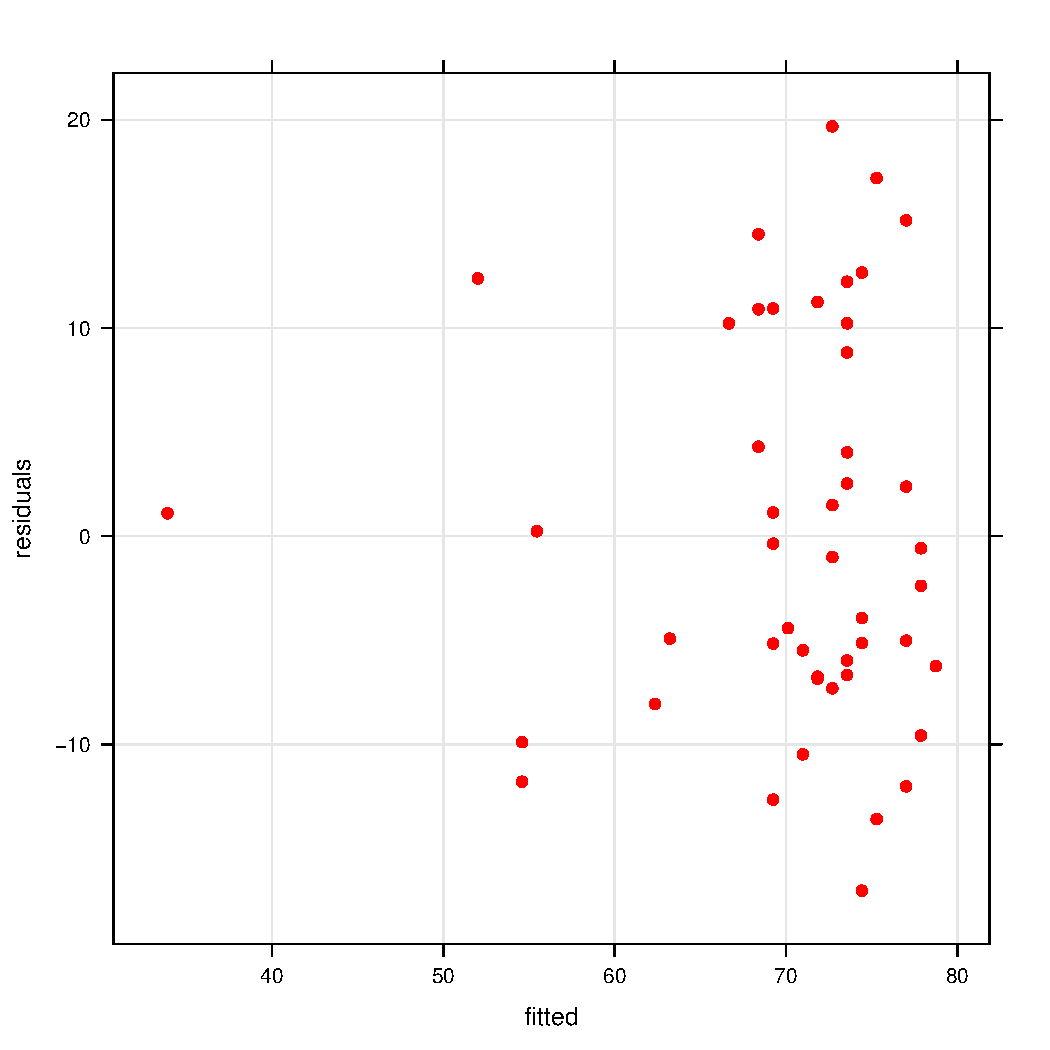
\includegraphics[height=0.7\textheight]{figs/xyplotS4.pdf}
\end{center}
\end{frame}
\end{document}